\title{Registration Form in PicoLisp}
\author{Henrik Sarvell}
% Use \authorrunning{Short Title} for an abbreviated version of
% your contribution title if the original one is too long
\institute{\texttt{hsarvell@gmail.com}}
%
% Use the package "url.sty" to avoid
% problems with special characters
% used in your e-mail or web address
%


\maketitle

\begin{abstract}
  This article describes how to build a \emph{website registration
    form} with PicoLisp.   
\end{abstract}

\section{Prerequisites}
\label{sec:registration-form}

Finally, the registration form! Not really for beginners but anyway…

If you are new to Pico Lisp you might want to check out
\href{http://www.prodevtips.com/2008/03/28/pico-lisp/}{the first article in the series} and move ``upwards''. Apart from that this tutorial builds
upon two earlier articles.
\href{http://www.prodevtips.com/2008/07/01/regular-expressions-in-pico-lisp/}{Regular expressions} and
\href{http://www.prodevtips.com/2008/07/17/templating-in-pico-lisp/}{templating}.

\begin{figure}[H]
  \centering
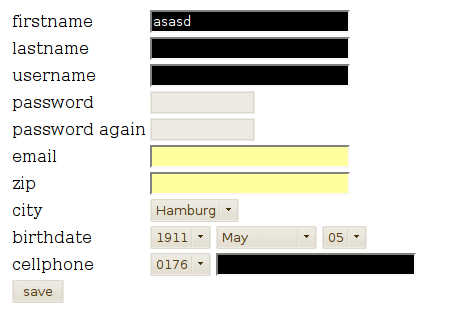
\includegraphics[scale=.6]{graphics/pico_reg_form.png}  
\end{figure}

I've changed the background color to black and the text to white just as
a test to see if the CSS was loading properly. Let's walk in order of
execution, first out is \textbf{main.l}:

\section{Walk through the \texttt{main.l} library}
\label{sec:registration-form}

\begin{wideverbatim}
(load "lib/http.l" "lib/xhtml.l" "lib/form.l" "lib/ps.l"
 "lib/adm.l" "lib/misc.l" "lib/rgx.l" "lib/tpl.l")
(setq *BP "projects/tpl-test/")
(setq *Css (pack *BP "css/styles.css"))
(load 
 (pack *BP "models/er.l") 
 (pack *BP "helpers/global-helpers.l"))

(de main () 
  (pool (pack *BP "db/test.db")))
    
(de start ()
  (app)
  (setq Tpl (new '(+Tpl) *BP))
  (assign> Tpl 'title "Registration Form")
  (parse> Tpl 'index)
  (compRun> Tpl)
  (out> Tpl))                  

(de go () 
   (server 8080 "@start"))
\end{wideverbatim}

So apart from the libraries we load \textbf{er.l} and \textbf{global-helpers.l},
\textbf{rgx.l} and \textbf{tpl.l} are the two libraries whose explanations I link to
above.

We load the database with pool initially because we start the server
with: \textbf{.p/ dbg.l projects/tpl-test/main.l -main -go.}

And go is of course responsible for starting the server on
\texttt{port 8080} and running start.

The start function will first start the session with app, create the
template object with our base path \texttt{*BP} and assign a title,
parse the template, compile it, run it and finally print it to the
browser.

Let's take a look at the template:

\begin{wideverbatim}
<html>
<head>
<title> <% get title %> </title>
<base href="<% bPath %>"/>
<link rel="stylesheet" href="<% path cssDir %>styles.css" type="text/css" >
</head>
<body>
<% gui reg-form %>
</body>
</html>
\end{wideverbatim}

There are some new things here since we went through the
\href{http://www.prodevtips.com/2008/07/17/templating-in-pico-lisp/}{template
  class}, but not much:

\begin{wideverbatim}
(dm path> (Var)
   (pack (srcUrl) (get This Var)))

(dm bPath> ()
   (baseHRef))
\end{wideverbatim}

The result could look like this:


\begin{wideverbatim}
<base href="http://localhost:44148/"/>
<link rel="stylesheet"
      href="http://localhost:8080/projects/tpl-test/css/styles.css" 
type="text/css" >
\end{wideverbatim}

So \texttt{baseHRef} outputs \href{http://localhost:44148}{http://localhost:44148} and
*srcUrl*\href{http://localhost:8080/}{http://localhost:8080/}, great. The reason for the base tag is
that the \href{http://software-lab.de/app.html}{GUI framework} needs it.
The port number keeps track of each session and is unique for that
nsession.


\section{Walk through the \texttt{er.l} library}
\label{sec:registration-form}

Before we start with the form itself let's go through the
\textbf{er.l} file and \textbf{global-helpers.l}, first \texttt{er.l}:

\begin{wideverbatim}
(extend +Entity)
(dm asSelect> ()
    (collect (: lbl) This NIL T (: lbl)))

(class +Member +Entity)
(rel fname    (+Need +Sn +Idx +String))
(rel lname    (+Need +Sn +Idx +String))
(rel uname    (+Need +Key +Sn +Idx +String))  #min 6 chars
(rel pwd      (+Need +String))                #min 6 chars
(rel zip      (+Need +Idx +String))           #min 5 chars, numerical
(rel city     (+Link)(+City))                 #lives in a city
# min 7 digits for validation but we store min 11 digits 
# (as is, no loc formatting)    
(rel cellnr   (+Need +Ref +String))  
# has to validate as proper email address
(rel email    (+Need +Key +Idx +String))     
(rel bdate    (+Need +Ref +Date))             #birthdate

\end{wideverbatim}

\begin{wideverbatim}

(class +CellPrefix +Entity)
# will be used in the registration to create a complete cell number
(rel nr (+Ref +String))
(var lbl . nr)

(class +City +Entity)
(rel nm (+Ref +String))
(var lbl . nm)
\end{wideverbatim}

We've got a link to \texttt{+City} in the \texttt{+Member}. The
\texttt{asSelect>} method is responsible for fetching a list to be
used as a drop down. In the \texttt{+CellPrefix} case it is
\textbf{nr} of course, and in the \texttt{+City} case it's
\textbf{nm}. Actually pretty redundant since they only have one
relation but that could quickly change.


\section{Walk through the \texttt{global-helpers.l} library}
\label{sec:registration-form}

\texttt{Global-helpers.l} contains some extra validation logic and
generators:

\begin{wideverbatim}
(class +Gh)

(dm range> (Start End Pad) 
    (make 
     (for (N Start (>= End N) (inc N)) (link (pad Pad N)))))
    
(dm getMonths> () 
    (range> This 1 12 2))

(dm getDays> () 
    (range> This 1 31 2))

(dm getYears> (Min-age)
    (let curYear (curYear> This) 
      (range> This (- curYear 100) (- curYear Min-age) 0 )))

(dm curYear> () (car (date (date))))
\end{wideverbatim}

Trivial stuff to generate various drop downs. Note \texttt{pad} to
get \texttt{01}, \texttt{02} etc.


\begin{wideverbatim}
(class +EmailField +TextField)
    
(dm chk> ()
  (ifn 
     (match> '+Rgx (super) '((word > 0) "{at}" (dmn > 0) "." (ltr > 2 < 5))) 
     ,"email-expected" 
     (super)))
    
(class +AlNum +TextField)

(dm chk> ()
  (ifn (alnum> '+Rgx (val> This)) ,"alnum-expected" (super)))
\end{wideverbatim}

So we create a new \texttt{+EmailField} and \texttt{+AlNum} based
on the basic \texttt{+TextField}. The main thing here is the
\texttt{chk>} method that is called automatically by the GUI logic
in order to check if a value is OK or not. The \texttt{+Rgx} stuff has
already been covered. Note the comma (\texttt{,}) It's a shortcut
for the localization logic, it will lookup the keys for translations
in translation files if they are provided, currently not though. Check
out the the
\href{http://www.prodevtips.com/2008/04/11/more-oo-in-pico-lisp/}{OO
  tutorial} for more info on \texttt{super} above, and
\texttt{extra} used below.


\begin{wideverbatim}
(class +MinLen)

(dm T (MinLen . @)
  (=: minLen MinLen)
  (pass extra))

(dm chk> ()
  (ifn 
     (>= (length (val> This)) (: minLen)) 
     (pack ,"minlen-1" (: minLen) ,"minlen-2") 
     (extra)))
\end{wideverbatim}

The minimum length logic, it does not inherit from something else but
is setup to work with other classes in a horizontal fashion. Note the
use of \texttt{,”minlen--1″ (: minLen) ,”minlen--2″}. We need this to
account for differing minimum lengths in the error message.

\begin{wideverbatim}
(class +PwdCheck)

(dm T (PwdGet . @)
  (=: pwdGet PwdGet)
  (pass extra))

(dm chk> ()
  (ifn (= (eval (: pwdGet)) (val> This)) ,"password-mismatch" (extra)))
\end{wideverbatim}

Also designed to be prefix class only. We simply check if the passwords
match.


\section{The registration form}
\label{sec:registration-form}

It's time for the registration form which is a biggie, I've uploaded it
\href{http://www.prodevtips.com/wp-content/uploads/2008/08/reg-form.l}{here}
if you want to see the whole thing at once. It will be chopped up below
in a from top to bottom fashion.

\begin{wideverbatim}
(action
    (let E (loc "*Err" err) 
       (set E (head 1 (val E))))
    (form NIL
       (unless *Post (=: obj (new! '(+Member))))
       (<table> NIL NIL NIL
          (<row> NIL ,"firstname" (gui '(+E/R +TextField)   
                '(fname : home obj) 10))
          (<row> NIL ,"lastname"  (gui '(+E/R +TextField) 
                 '(lname : home obj) 10))
          (<row> NIL ,"username"  (gui '(+E/R +MinLen +AlNum) 
                 '(uname : home obj) 6 10))
\end{wideverbatim}

Having everything be an argument to the action function is a requirement
for the GUI to work.

The first thing we do is override the default behavior of displaying
validation errors for all fields at once. We get the \texttt{*Err}
list from the err function defined in \texttt{form.l} line 207. After
that we extract and use the first error (if there are any).

The second thing we do is to build an empty \texttt{+Member} object
which will be available through \texttt{(: home obj)}. You might
notice the use of \textbf{new}!, what happens if the user just
navigates away you might think, there will be a lot of empty bullshit
in the database won't it? Sure, and they can be cleared out by running
a cron job every day or continuously although it consumes more
resources. Since we work with a new! object there will be no need for
future commits, from now on everything that happens happens on disk,
not memory.

We build the layout in a table where each call to
\texttt{\textless{}row\textgreater{}} will create new rows and tds.
Notice the calls to \texttt{gui}, apparently \texttt{+E/R} needs the
\texttt{'(fname home obj)} list and \texttt{+TextField} the 10 number
(the size of the field).

Our first custom prefix classes comes in the form of \texttt{+MinLen}
and \texttt{+AlNum} which takes 6 and 10 respectively (remember that
+AlNum is just a \texttt{+TextField} with extra validation attached to
it).

\begin{wideverbatim}
(<row> NIL ,"password"       
   (gui 
      '(+E/R +PwdCheck +MinLen +PwField) 
      '(pwd : home obj) 
      '(val> (: home pwd2)) 6 10))
(<row> NIL ,"password again" (gui 'pwd2 '(+PwField) 10 ))
(<row> NIL ,"email" (gui '(+E/R +EmailField)       '(email : home obj) 10))
(<row> NIL ,"zip"   (gui '(+E/R +MinLen +NumField) '(zip : home obj) 6 10))
(<row> NIL ,"city"  (gui '(+E/R +TextField)        '(city : home obj) (asSelect> '+City)))
\end{wideverbatim}

Note that the code has been indented to save horizontal space, in
reality it's just a continuation of the above code.

\texttt{+PwdCheck} will work with \texttt{'(val> (: home pwd2))} as
input, yes it's the value of the ``password again'' field.

The city \texttt{+TextField} will get the result of the \texttt{(asSelect>
'+City)} call as it's input, note the lack of a quote (\textbf{'}). So
we evaluate and get the list of cities which will turn the field into
a drop down instead of a normal text field.

\begin{wideverbatim}
(<row> NIL ,"birthdate" 
   (<div> 
      (gui '(+E/R +Fmt +Chart) '(bdate : home obj)
         '((Dat) (list (date Dat)))
         '((Lst) (and (caar Lst) (cadar Lst) (caddr (car Lst)) (date (car Lst))))
         3 )
      (gui 1 '(+TextField) (getYears> '+Gh 18))
      (gui 2 '(+Map +TextField)
         (make 
            (for (I . M) *MonFmt 
               (link (cons M I))))
         *MonFmt)
      (gui 3 '(+TextField) (getDays> '+Gh))))
\end{wideverbatim}

It's starting to get tricky. Remember that we use \texttt{+Date} for
the birth date so we need some way of getting it to prepopulate three
consecutive drop downs, and be inserted by getting the data in all of
them. Actually we are just updating the empty object we created at the
top all the time but insert might be a more proper wording since we
are replacing nothing with something.

The \texttt{+Fmt} is class will take care of getting and setting the
date, the first function \texttt{'((Dat)\dots{})} will \texttt{set>}
and the second one \texttt{'((Lst)\dots{})} will be our \texttt{val>}
function.

The \texttt{+Chart} prefix is responsible for handling our 3 date drop
downs and will therefore take 3 as its single argument. The
constituent gui elements need to know where they are in this list,
hence 1, 2 and 3 as the first argument. The second drop down will
display the months of the year by working with the global
\texttt{*MonFmt} which will contain the full names based on which
location we have selected. Since we haven't chosen a location they
will default to their English names. Come to think of it this piece of
code should have been put in global helpers since month drop downs are
pretty common.

\begin{wideverbatim}
(<row> NIL ,"cellphone" 
   (<div> 
      (gui '(+E/R +Chart) '(cellnr : home obj) 2 
         '((Str)
             (let Len 
                (length 
                   (Find '((P) (pre? P Str)) (asSelect> '+CellPrefix)))
                (setq Str (chop Str))
                (list 
                   (list (pack (cut Len 'Str)) (format (pack Str))))))
         '((Lst) (pack (caar Lst) (cadar Lst))))
      (gui 1 '(+TextField) (asSelect> '+CellPrefix))
      (gui 2 '(+MinLen +NumField) 7 10 )))
(<row> NIL (gui '(+Button) ,"save" '(url "@start"))))))
\end{wideverbatim}

Here we pass two extra set and get functions to the \texttt{+Chart}
class directly instead. The first one is needed due to the fact that
it will recieve for instance a string looking like
\texttt{01766587436}. It then needs to cut the string up to get a list
looking like this: \texttt{(0176 6587436)}, in order to repopulate on
for instance validation failure. The problem is that some mobile phone
prefix numbers can have five digits in Germany, ouch. That's why we
need to determine the length first, otherwise we could end up with the
wrong numbers.

Finally the \texttt{+Button} will post the form back to the start
function which in turn contains this function. The error logic at the
top of the form could be used to confirm a successful post by
displaying a new page or message. No error \texttt{==} success.

